\labday{21 March 2023}

\experiment{PPDr}

When the output of the trigger PMT was observed with a scope, the signal looked extremely noisy, and repeated at around \SI{5.6}{\kilo\hertz}. Figure \ref{fig:PPDScopeNoise} shows this. I was unable to determine as to whether this was the laser or the PMT, however the laser was visibly damaged so this was the suspected cause at this stage.

\begin{figure}[H]
\begin{center}
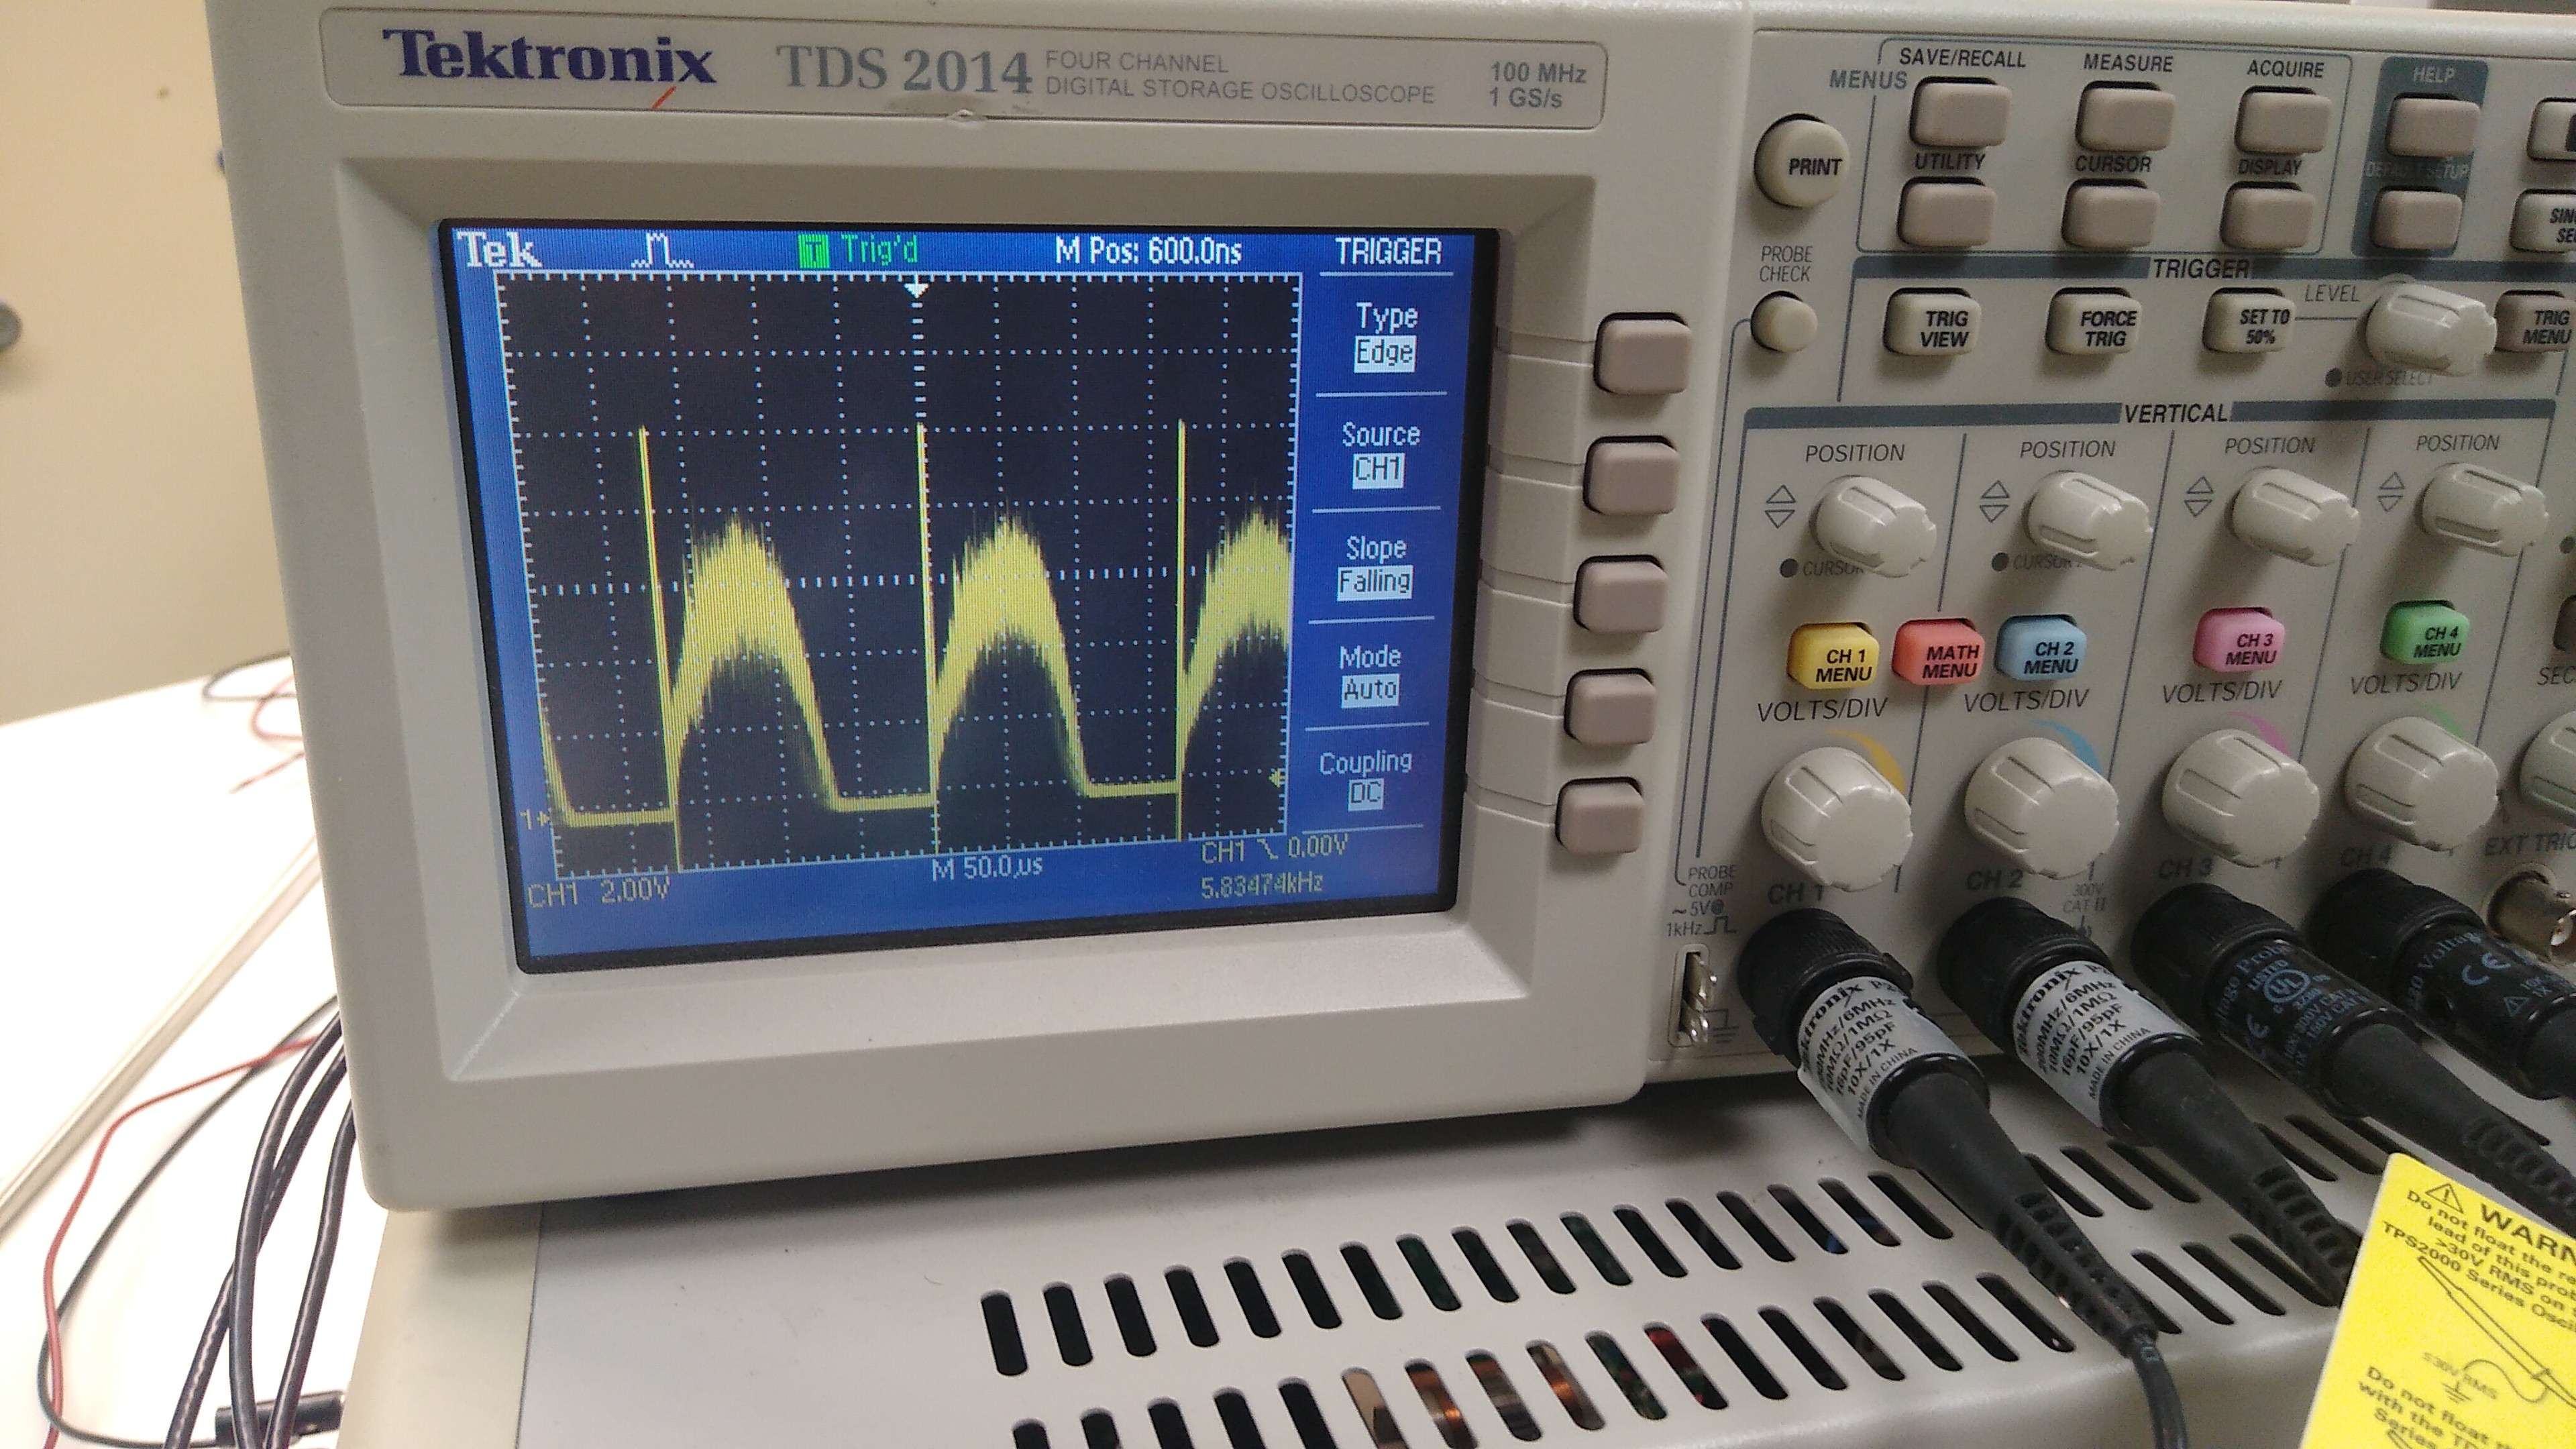
\includegraphics[width=0.5\linewidth]{Figures/PPDScopeNoise}
\end{center}
\caption{Noise after campaign with old laser.}
\label{fig:PPDScopeNoise}
\end{figure}

When an object was inserted into the optics chamber, the output resembled a square wave. This is shown in Fig. \ref{fig:PPDScatterOutput}.

\begin{figure}[H]
\begin{center}
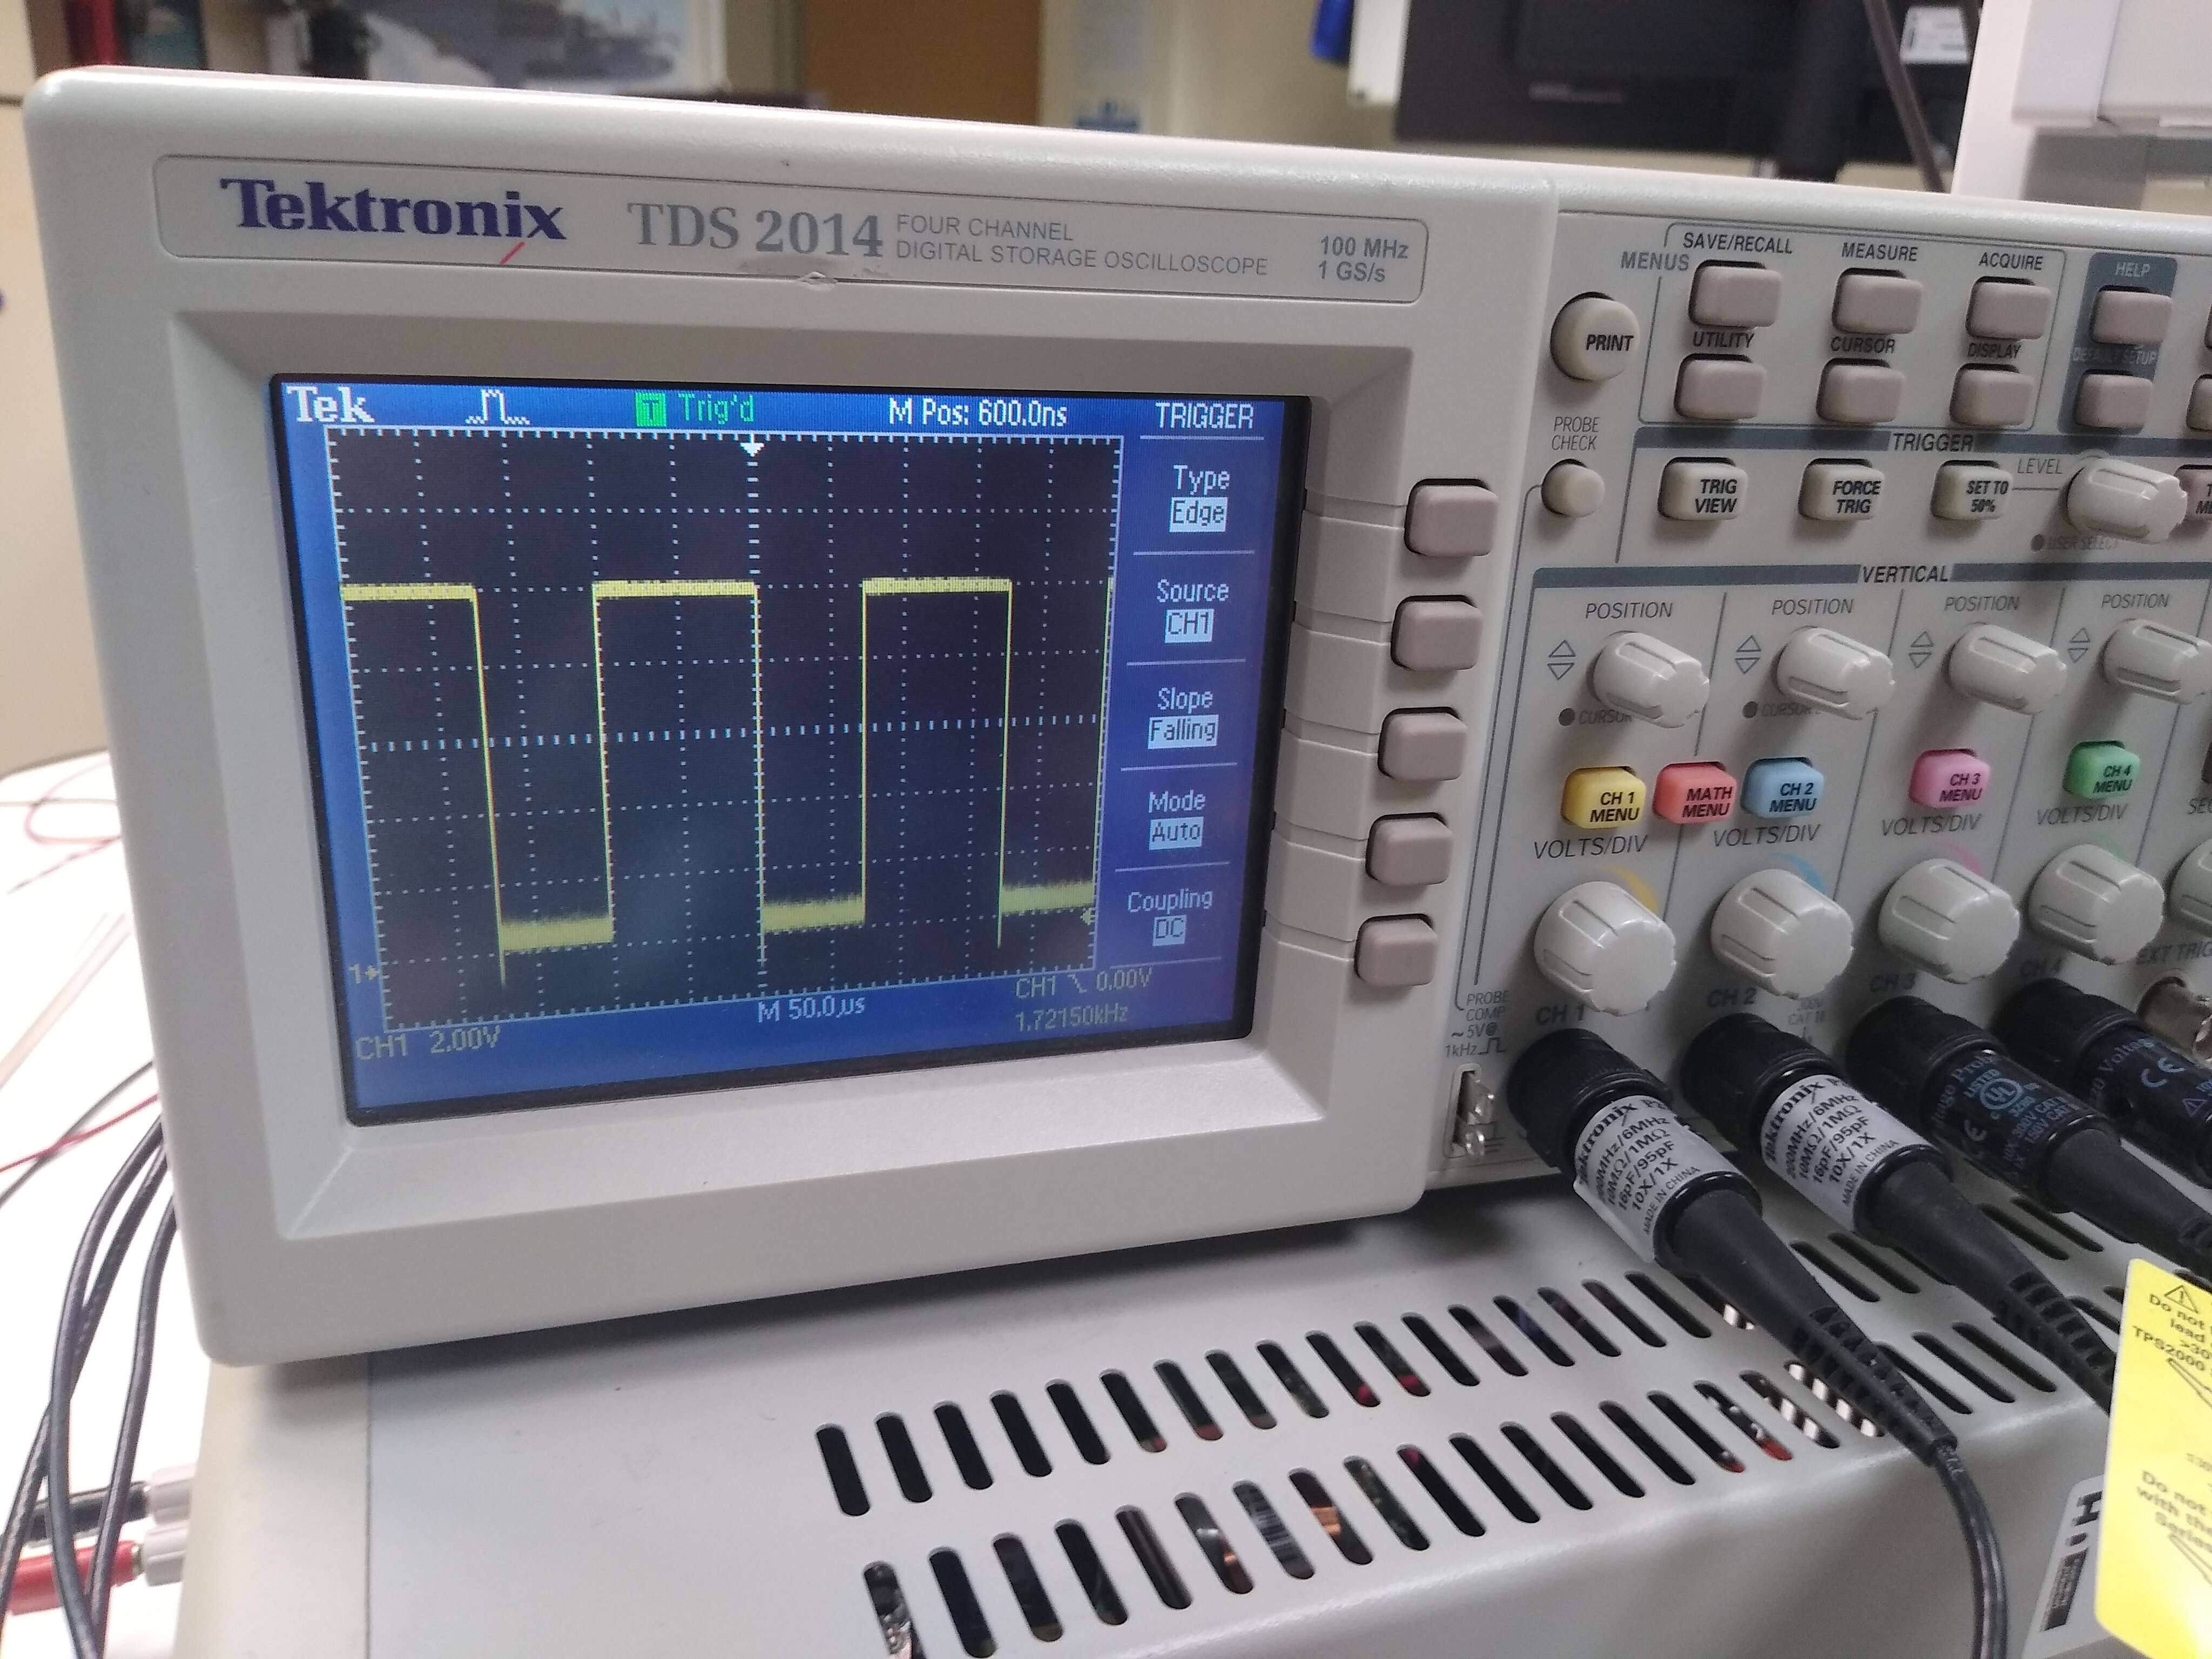
\includegraphics[width=0.5\linewidth]{Figures/PPDScatterOutput}
\end{center}
\caption{Noise after campaign with old laser and object in beam.}
\label{fig:PPDScatterOutput}
\end{figure}

The beam was also visibly dimmer, which would explain the lower image intensity. A pulse generator was configured to trigger the camera with a simulated 5 particles per second, each with a \SI{10}{\micro\second} pulse width. The camera triggering was unreliable, oftentimes exhibiting the characteristics of a "busy port".

It was decided that a new laser was the preferable option. A replacement CrystaLaser \SI{532}{\nano\metre} at \SI{150}{\milli\watt} was located.
